% ****** Start of file apssamp.tex ******
%
%   This file is part of the APS files in the REVTeX 4.1 distribution.
%   Version 4.1r of REVTeX, August 2010
%
%   Copyright (c) 2009, 2010 The American Physical Society.
%
%   See the REVTeX 4 README file for restrictions and more information.
%
% TeX'ing this file requires that you have AMS-LaTeX 2.0 installed
% as well as the rest of the prerequisites for REVTeX 4.1
%
% See the REVTeX 4 README file
% It also requires running BibTeX. The commands are as follows:
%
%  1)  latex apssamp.tex
%  2)  bibtex apssamp
%  3)  latex apssamp.tex
%  4)  latex apssamp.tex
%
\documentclass[%
 reprint,
%superscriptaddress,
%groupedaddress,
%unsortedaddress,
%runinaddress,
%frontmatterverbose,
%preprint,
%showpacs,preprintnumbers,
%nofootinbib,
%nobibnotes,
%bibnotes,
 amsmath,amssymb,
 aps,
pra,
%prb,
%rmp,
%prstab,
%prstper,
%floatfix,
]{revtex4-1}

\usepackage{graphicx}% Include figure files
\usepackage{dcolumn}% Align table columns on decimal point
\usepackage{bm}% bold math
\usepackage{enumitem}
% Stuff for Mogens' nice figure
\usepackage{braket}
\usepackage{tikz}


% Stuff for showing the algorithms
\usepackage{algorithm}
\usepackage[noend]{algpseudocode}

\newcommand{\dif}[2]{\frac{\text{d} #1}{\text{d} #2}}
\newcommand{\diff}[2]{\frac{\partial #1}{\partial #2}}
\DeclareMathOperator*{\argmin}{arg\,min}

\newcommand{\procspie}{Proceedings of the SPIE}
%\usepackage{hyperref}% add hypertext capabilities
%\usepackage[mathlines]{lineno}% Enable numbering of text and display math
%\linenumbers\relax % Commence numbering lines

%\usepackage[showframe,%Uncomment any one of the following lines to test
%%scale=0.7, marginratio={1:1, 2:3}, ignoreall,% default settings
%%text={7in,10in},centering,
%%margin=1.5in,
%%total={6.5in,8.75in}, top=1.2in, left=0.9in, includefoot,
%%height=10in,a5paper,hmargin={3cm,0.8in},
%]{geometry}

\begin{document}

%\preprint{APS/123-QED}

\title{Gradient-Based Optimal Control of Quantum Many-body Systems in Optical Lattices}% Force line breaks with \\

\author{F. S. M\o ller}
\author{J. J. W. H. S\o rensen}
\author{J. F. Sherson}
\affiliation{Aarhus University}
\email{sherson@phys.au.dk}
\date{\today}% It is always \today, today,
             %  but any date may be explicitly specified

\begin{abstract}
Abstract ...


\end{abstract}

\maketitle


\section{Introduction}

\textbf{What is control used for and why is it important?}
\begin{itemize}
	\item
	Adiabatic solutions too slow / systems too complex to describe analytically

	\item
	Realize cold complex systems/configurations
	
	\item
	State preparation 
\end{itemize}


\textbf{What are the previous examples of optimal control?}
\begin{itemize}
	\item
	Examples of CRAB
	
	\item
	Examples of GRAPE/Krotov
	
	\item
	GROUP is CRAB+GRAPE
	
	\item
	Complex systems require tensors, tDMRG. So far only CRAB, however tDMRG propagator has analytical  
\end{itemize}


\textbf{What is done for this paper?}
\begin{itemize}
	\item
	Investigates the phase transition in the Bose-Hubbard model. This system is of interest as it is complex enough to warrant a tensor description, while the Mott is a central component of several experiments.

	\item
	Derived GRAPE gradient for tDMRG propagator. Choosing diagonal control Hamiltonian causes all higher order contributions to vanish.
	
	\item 
	Illustrates how GROUP compares to other methods in optimizing tensor networks.
\end{itemize}

During the last decade great improvements in the experimental cold atoms toolbox have been realized, which has enabled a large degree of control  of quantum systems. Cold quantum gases provides a powerful experimental tool, as various Hamiltonians can be mapped to the physical systems, while external fields enable manipulations of the dynamics and properties of the atoms. Gradually, quantum systems realized are becoming too complex to accurately describe analytically, whereby suboptimal control schemes of the external fields have become one of the main limiting factors in achieving high-fidelity configurations. Furthermore, state transfers required for the preparation of quantum many-body systems often rely on adiabatic protocols resulting in needlessly long experimental cycles, in which the quantum system is vulnerable to heating or decoherence.

Quantum optimal control is a framework enabling the design of control strategies that achieve the desired dynamics (REPLACE). 
In quantum optimal control a common method of optimizing the control sequence is formulating the desired dynamics in terms of a minimization problem. Thereby, the quantum optimal control framework can utilize many of the methods developed in mathematical optimization theory. Two powerful algorithms within the framework are the GRadient-Ascent Pulse Engineering (GRAPE) and Krotov's method, which have been used in EXAMPLES. Both methods utilize the gradients of some cost functional to find the optimal control sequence. Derivative-based algorithms generally converge faster than those methods not using the additional information of the gradient, however, they are limited by the efficiency at which the derivative can be computed. 
Derivative-free algorithms typically struggle optimizing a large set of parameters. Therefore, an alternative approach is parameterizing the control in a reduced basis such as the Chopped RAndom Basis (CRAB). The CRAB method has previously been used in conjunction with the Nelder-Mead algorithm to find optimal control sequences for highly complex quantum many-body systems, whose dynamics must be simulated through tensor-network-based techniques such as the time-dependent Density Matrix Renormalization Group (tDMRG). Evaluating cost-derivatives in systems described by tensor networks has so far been considered too inefficient.
The GRadient Optimization Using Parametrization (GROUP) method introduced in REF combines a chopped basis description of the control with the gradient-based optimization of GRAPE. A characterization of the method on solving optimal control problems regarding Bose-Einstein condensates manipulated in an atom chip trap revealed that GROUP outperformed all the previously mentioned algorithms in terms of convergence rate and achieved result. 

In this paper we derive the chopped basis parametrized gradient for systems described by tensor networks. Additionally we show that the propagator expansion required for the tDMRG algorithm causes higher order contributions to the GRAPE gradient to vanish if one chooses a diagonal control Hamiltonians. Thereby the precision of the cost derivative is solely dependent on the expansion error.
The method is benchmarked in the context of crossing the superfluid to Mott-Insulator phase transition of the Bose-Hubbard model. Preparing a Mott-Insulator with very high fidelity is important, as the state constitutes the basis of many experiments (EXAMPLES). Furthermore, the phase transition of the Bose-Hubbard model has previously been investigated using Nelder-Mead with CRAB \cite{doria2011optimal,van2016optimal}.
To ensure a proper comparison between the two methods, we solve the exact same optimization problem using both GROUP and Nelder-Mead with CRAB.
\section{The Control Problem}

In quantum optimal control a given state transfer or unitary is achieved by dynamically manipulating a system through a time-dependent Hamiltonian
\begin{equation}
	\hat{H} =  \hat{H}_0 + \sum_{n = 1}^{m}  \hat{H}_n (u_n(t)) \; ,
	\label{eq:ControlHamiltonians}
\end{equation} 
where $\hat{H}_0$ is an uncontrollable drift, while $\hat{H}_n$ can be adjusted through the control functions $u_n(t)$. Here, the system under investigation is a Bose-Einstein condensate placed in a one-dimensional optical lattice. The system is well described by the Bose-Hubbard model
\begin{equation}
	\hat{H} = - J \sum_{\langle i,j \rangle} \hat{a}_{i}^{\dag} \hat{a}_{j} + \frac{U}{2} \sum_{i} \hat{n}_i \left( \hat{n}_i -1 \right) \; ,
\end{equation}
where $J$ and $U$ are the tunneling and interaction matrix elements respectively, which depend on the depth of the lattice wells. The matrix elements are in units of recoil energy $E_{\mathrm{rec}} = \frac{\hbar ^2 k^2}{2 m}$, where $m$ is the mass of the atoms of the BEC, and $k$ is the photon wave number of the light forming the optical lattice.
Experimentally the Bose-Hubbard model is often realized using ultracold gases of Rb-87 and lattice wavelengths of $\lambda = 1064 \: \mathrm{nm}$. Thus, the recoil energy is on the order of ... (units of ??)

In this work we examine the superfluid to Mott-insulator phase transition of the Bose-hubbard model, which can be crossed solely by varying the fraction $U/J$. The Bose-Hubbard system is controlled experimentally by adjusting the intensity of the lasers constituting the optical lattice, which in turn varies the depth of the lattice. Alternatively, the interaction $U$ can be expressed in units of the tunneling $J$, whereby the interaction term of the Bose-Hubbard model constitutes the control Hamiltonian, while the tunneling can be modeled as the drift.

The desired dynamics can be achieved by formulating a state transfer problem, $\ket{\psi_0} \to \ket{\psi_{\mathrm{target}}}$, where the initial state $\ket{\psi_0}$ is a ground state in the superfluid phase, while the desired target-state $\ket{\psi_{\mathrm{target}}}$ is a ground state in the MI phase. Thus, the problem can be expressed as the minimization of the cost function
\begin{equation}
	J = \frac{1}{2} \left( 1-|\braket{\psi_{\mathrm{target}} | \psi (T)}|^2 \right) \; ,
	\label{eq:infidelityCost}
\end{equation}
where $T$ is the duration of the control sequence. Since the control functions determine the time evolution, one must find the set of controls bringing the final state as close as possible to the target state. In practice, very few optimal control problems can be solved analytically, however, expressing the problem as a minimization enables the use of well established frameworks derived in mathematical optimization theory.
\section{Tensor-Network Descriptions}

For complex many-body systems the Hilbert space grows too large for standard descriptions of states. Due to the combinatorial nature of the Bose-Hubbard model its corresponding Hilbert space scales exponentially with the system size. Matrix Products States parametrize states as networks of tensors.

Mention relation to lattices ...

A general state can be decomposed into a tensor network through a series of Schmidt decompositions, where eigenstates barely contributing to the overall state can be omitted resulting in a truncation of the dimensions of the tensor. The truncation along with an area law scaling of entropy with the system results in matrix product states only requiring to consider a small corner of the full Hilbert space.

Several methods exists for time-evolving tensor networks, however, most of them are variants of the same core ideas originally derived from the DMRG algorithm. The tDMRG algorithm employs a Trotter expansion of the propagator in order to evolve the state by applying a series of site-specific gate operations to the state.

Describe tailored tDMRG algorithm ...
\section{Quantum Optimal Control}

GRADIENT MOTIVATION ....

GRAPE is a popular method for calculating gradients of optimal control cost functionals \cite{khaneja2005optimal}. The method has successfully been applied to EXAMPLES systems. In GRAPE the control function is discretized in time-steps of  $\Delta t$. While the gradient of the cost function in the original algorithm was derived to $O(\Delta t ^2)$ precision, a series of higher order corrections were added in \cite{de2011second}. The derivative of the cost function \eqref{eq:infidelityCost} with respect to the time-discretized control function is
\begin{equation}
	\frac{\partial J}{\partial u_n (t_j)}  = - \Re \Braket{\chi (t_j) | i  \frac{\partial \hat{\mathcal{U}}_{t_j}}{\partial u_n (t_j)} | \psi (t_{j-1})} \; , \label{eq:CostDeriv}
\end{equation}
where $\ket{\chi (T)} \equiv i \ket{\psi_{\mathrm{target}}} \braket{\psi_{\mathrm{target}} | \psi (T)}$ must be propagated back in time to obtain $\ket{\chi (t_j)}$.
The derivative of the propagator with respect to the control is given by
\begin{align}
	\frac{\partial \hat{\mathcal{U}}_{j}}{\partial u_n (t_j)} &= e^{-i \hat{H} (u_n (t_j)) \Delta t} \nonumber \\ 
	 \times \sum_{k = 0}^{\infty } &  \frac{i^{k-1} \Delta t^{k+1}}{(k+1)!} \left[ \hat{H} (u_n (t_j)) , \frac{\partial \hat{H} (u_n (t_j))}{\partial u_n (t_j)}  \right]_k \; , \label{eq:PropDeriv}
\end{align}
where the zeroth order term of the recursive commutator produces the gradient of the original GRAPE algorithm.

Calculating the propagator after each control update is an expensive procedure, as exponentiating the Hamiltonian \eqref{eq:ControlHamiltonians} is non-trivial. The Hamiltonian can be exponentiated term-wise through the Suzuki-Trotter expansion
\begin{equation}
		e ^{( \hat{H}_n + \hat{H}_0  ) \delta } = e^{  \hat{H}_n \delta /2  } e^{ \hat{H}_0 \delta } e^{ \hat{H}_n \delta /2 } + O(\delta^3) \; , \label{eq:SuzukiTrotter}
\end{equation}
where the error is due to any non-commutativity of the operators.
Thus, the propagator can be updated efficiently, as only $e^{ \hat{H}_n \delta /2 }$ must be re-calculated as $u_n (t)$ is updated. Additionally, Trotter-expanding the propagator is a necessary step for conducting time-evolution through the tDMRG algorithm. 

Further improvements in the cost of computing the propagator can be found if $\hat{H}_n$ is diagonal, as the exponentiation becomes trivial. Choosing a diagonal control Hamiltonian also has profound impact on the  derivative of the propagator, as all higher-order contributions vanish.\\
Consider a Suzuki-Trotter expanded propagator, where $\hat{H}_n (u_n (t))$ is evaluated at either side of the time-step for increased accuracy
\begin{align}
	\hat{\mathcal{U}}_{j}^{\mathrm{ST}} &\equiv e^{ -i  \hat{H}_n (u (t_j)) \Delta t /2 } \; e^{ -i \hat{H}_0 \Delta t } \; e^{ -i  \hat{H}_n (u (t_{j-1}))  \Delta t /2 } \\
	& \equiv \hat{\mathcal{U}}_{j}^{(n)} \hat{\mathcal{U}}_{j}^{(0)} \hat{\mathcal{U}}_{j-1}^{(n)} \; .
\end{align}
Both $\mathcal{U}_{j}^{\mathrm{ST}}$ and $\mathcal{U}_{j+1}^{\mathrm{ST}}$ contribute to the cost derivative due to the split-step of the control.
The derivative of $\mathcal{U}_{j}^{\mathrm{ST}}$ according to eq. \eqref{eq:PropDeriv} is
\begin{align}
	\frac{\partial \hat{\mathcal{U}}_{j}^{\mathrm{ST}}}{\partial u_n (t_j)} &=  \frac{\partial \hat{\mathcal{U}}_{j}^{(n)}}{\partial u_n (t_j)} \hat{\mathcal{U}}_{j}^{(0)} \hat{\mathcal{U}}_{j-1}^{(n)} \nonumber \\
	&= e^{ -i  \hat{H}_n (u (t_j)) \Delta t /2 } \left( -i \hat{H}_n (u_n (t_j)) \Delta t /2 \right) \hat{\mathcal{U}}_{j}^{(0)} \hat{\mathcal{U}}_{j-1}^{(n)} \nonumber \\
	&= \left( -i \hat{H}_n (u_n (t_j)) \Delta t /2 \right) \hat{\mathcal{U}}_{j}^{\mathrm{ST}} \; . \label{eq:STpropderiv1}
\end{align}
Since $\hat{H}_n$ is diagonal, the recursive commutator is vanishing for $k > 0$, which causes all higher-order contributions to the derivative of the propagator to drop out.\\
Likewise, the derivative of the second propagator is
\begin{equation}
	\frac{\partial \hat{\mathcal{U}}_{j+1}^{\mathrm{ST}}}{\partial u_n (j)} =  \hat{\mathcal{U}}_{j+1}^{\mathrm{ST}} \left( -i \hat{H}_n (u_n (t_j)) \Delta t /2 \right) \; . \label{eq:STpropderiv2}
\end{equation}
Inserting the derivatives of eq. \eqref{eq:STpropderiv1} and \eqref{eq:STpropderiv2} into the derivative of the cost (eq. \eqref{eq:CostDeriv}) yields
\begin{align}
	\frac{\partial J}{\partial u_n (t_j)} &= - \Re \Braket{\chi (t_j) |  \left(  \hat{H}_n (u_n (t_j)) \Delta t /2 \right) \hat{\mathcal{U}}_{j}^{\mathrm{ST}} | \psi (t_{j-1})} \nonumber \\
	& \quad - \Re \Braket{\chi (t_{j+1}) | \hat{\mathcal{U}}_{j+1}^{\mathrm{ST}} \left(  \hat{H}_n (u_n (t_j)) \Delta t /2 \right) | \psi (t_{j})} \nonumber \\
	&= - \Re \Braket{\chi (t_j) | \hat{H}_n (u_n (t_j)) \Delta t | \psi (t_{j})} \; . \label{eq:STcostgrad}
\end{align}  
Thus, the combination of the Suzuki-Trotter expansion and a diagonal control Hamiltonian eliminates all higher order contributions to the gradient. Thereby, the gradient of the cost is exact up to the order of the expansion.
\section{Numerical Optimization}

In GRAPE the dimension of the optimization space is $N = \lfloor T / \Delta t \rfloor$ due to the discretization. However, most optimal solutions require much fewer degrees of freedom than introduced in the discretization. Therefore, expanding the control in a proper basis can significantly reduce the dimension of the optimization space.
The GROUP algorithm utilizes the gradient-based optimization from GRAPE while employing a chopped basis parametrization 
\begin{equation}
	u(t) = u_0 (t) + S(t) \sum_{n=1}^{M} c_n f_n (t) \; . \label{eq:controlParametrization}
\end{equation}
Here, $f_n$'s are basis functions, the coefficients $c_n$'s are the optimization parameters, $u_0 (t)$ is the initial seed, and $S(t)$ is a shape function enforcing the boundary conditions of the original control. The derivative of the cost function in the parameterization can be derived using the chain rule
\begin{equation}
	\frac{\partial J }{\partial c_n} = \sum_{j = 1}^{N} \frac{\partial J }{\partial u(t_j)} S(t_j) f_n(t_j) \; . \label{eq:GROUPgradient} 
\end{equation}
The cost of calculating the partial derivative of eq. \eqref{eq:GROUPgradient} is dominated by the time evolution of the states $\psi$ and $\chi$ from eq. \eqref{eq:CostDeriv}. Hence, the computation time of the parametrized gradient is comparable to that of GRAPE.


MOTIVATE IPOPT (solve constrained, non-linear, multi-variable problems)

GENERAL (perhaps write using specific symbols for control problem)

Interior point methods solve barrier problems of the form
 \begin{align*}
	\min_{x , s} \; & \; f(x) - \mu \sum_{i=1}^{m} \log s_i \\
	\text{s.t.}  \; & \; c_E (x) = 0  \\ 
					& \; c_I (x) - s =0 \; ,
\end{align*}
where $c_E$ and $c_I$ are equality and inequality constraints of the problem, and the slack variables, $s$, transform the inequality constraints into equality constraints. The barrier term enforces the slack variables to remain positive, as the function diverges if any $s_i \to \infty$
The optimization Lagrangian of the problem reads
\begin{equation}
	\mathcal{L} = f(x) - \lambda ^T c_E (x) - \nu ^T (c_I (x) -s)
\end{equation}
where $\lambda$ and $\nu$ are the Lagrange multipliers of the equality and inequality constraints respectively. 
The Karush-Kuhn-Tucker conditions for the problem can be expressed in a single mapping
\begin{equation}
	F \equiv 
	\begin{bmatrix}
  \nabla_x f(x) - A_{E}^{T}(x) \lambda  - A_{I}^{T}(x) \nu \\
  S \nu - \mu e \\
  c_{E} (x)		\\
  c_{I} (x) - s 
  \end{bmatrix}
  = 0 \; ,
\end{equation}
where $A_E (x)$ and $A_I (x)$ are the constraint Jacobians. $S$ and $Z$ are defined as diagonal matrices with entries given by the vectors $s$ and $\nu$, while we let $e = (1 ,1 , \ldots , 1 )^T$.
Applying Newtons method to the non-linear problem given above yields
\begin{equation}
  \begin{bmatrix}
  \nabla_{xx} \mathcal{L} 	& 0 	& -A_{E}^{T}(x)	& -A_{I}^{T}(x)	\\
  0 						& Z 	& 0 			& S 			\\
  A_{E}(x) 					& 0 	& 0 			& 0				\\
  A_{I}(x) 					& -I	& 0				& 0				 
  \end{bmatrix}  
  \begin{bmatrix}
  p_x \\ p_s \\ p_{\lambda} \\ p_{\nu} 
  \end{bmatrix}
  = - F
\end{equation}
where $\left[ p_x , p_s , p_{\lambda} , p_{\nu} \right]$ is the Newton step direction.

This is a primal-dual system ...
For a sufficient small, positive barrier parameter $\mu$ the problem gas a locally unique solution denoted by the point $( x(\mu) , s (\mu) , \lambda (\mu) , \nu (\mu) )$. The main problem is solved by solving a series of subproblems for various values of $\mu$. The trajectory described by the local solution points is called the primal-dual central path, and it converges to $( x* , s* , \lambda* , \nu * )$ as $\mu \to 0$. (taken from book)

From GROUP the constraint Jacobian is given by ...
The Hessian $\nabla_{xx} \mathcal{L}$ is in practice too demanding to compute for control problems, however, it can be efficiently approximated using the L-BFGS method, which utilizes previous derivatives. Hence, it is important that the derivatives are very accurate, as a poor Hessian can reduce the speed of the optimization significantly. 

Optimal control problem often involve constraints ensuring the control parameters stay within a feasible limit
\begin{equation}
	 u_{min} (t_j) \leq u(t_j) \leq u_{max} (t_j) \; .
	 \label{eq:ControlConstraints}
\end{equation}
The parameterizing of eq. \eqref{eq:controlParametrization} does not alter the constraints, although additional constraints of the $c_n$ coefficients can be introduced. However, optimizing a constrained problem through its gradient requires the derivatives of the constraints expressed through a Jacobian, which will be affected by the parameterization. The matrix elements of the Jacobian of eq. \eqref{eq:ControlConstraints} parametrized by \eqref{eq:controlParametrization} are
\begin{equation}
	\boldsymbol{J}_{ij} = \frac{\partial u(t_i)}{\partial c_j} = S(t_i) f_j (t_i) \; . \label{eq:ConstraintJacobian}
\end{equation}
The Jacobian of the constraints has $N \times M$ entries, which remain constant throughout the optimization, whereby they can easily be retrieved.
\section{Results}


\begin{figure}[h!]
    \centering
    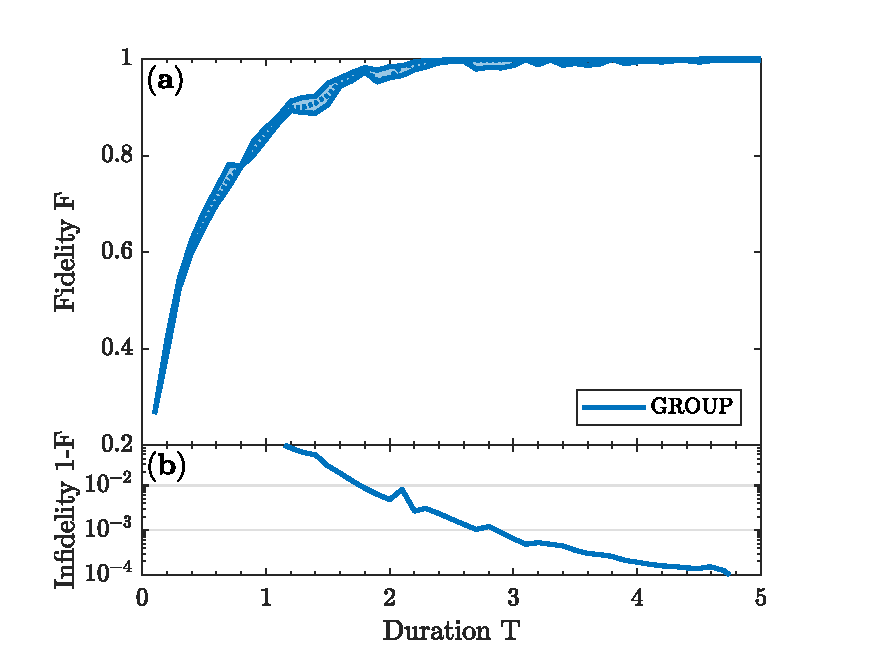
\includegraphics[width=0.45\textwidth]{Figures/FidelityDuration.pdf}
    \caption{\textit{Final fidelity obtained for optimal control at various durations. \textbf{(a)} the dotted line marks the median fidelity achieved, while the shaded area displays the $25\%$- and $75\%$-quartiles of the solutions. \textbf{(b)} the lowest infidelity achieved for each duration. }}
    \label{fig:FidelityDuration}
\end{figure}

\begin{figure}[h!]
    \centering
    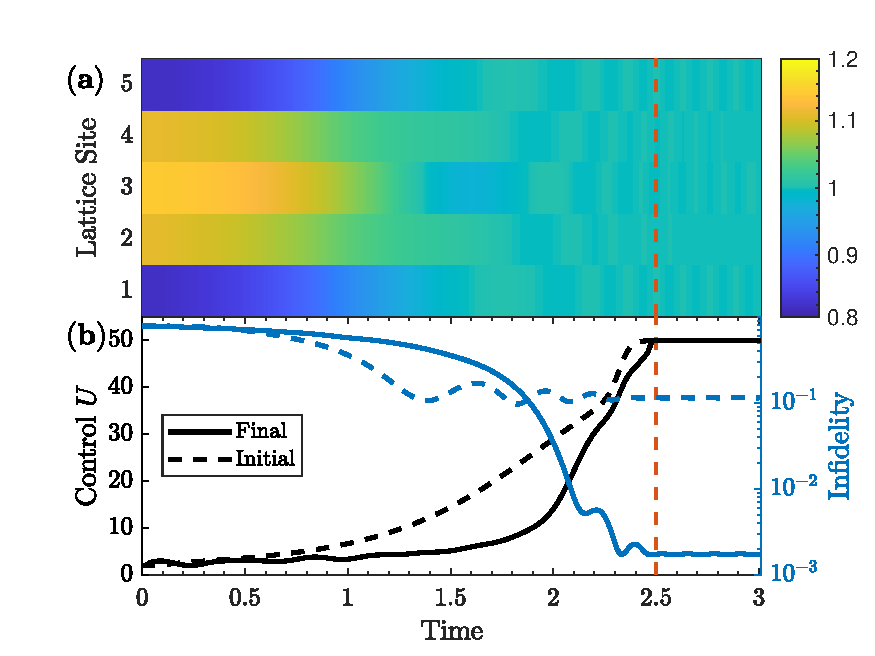
\includegraphics[width=0.45\textwidth]{Figures/OptRamp.pdf}
    \caption{\textit{Solution with highest fidelity achieved for duration $T = 2.5$. The dashed, red line marks the end of the duration, from which the system is further evolved using the final control value. \textbf{(a)} logarithmically scaled expectation value of the number operator, $\braket{\hat{n}_i}$, for each site, as the system is evolved according to the optimized ramp. \textbf{(b)} the initial and optimized ramp sequences along with the corresponding evolution of fidelities.}}
    \label{fig:OptRamp}
\end{figure}

\begin{figure}[h!]
    \centering
    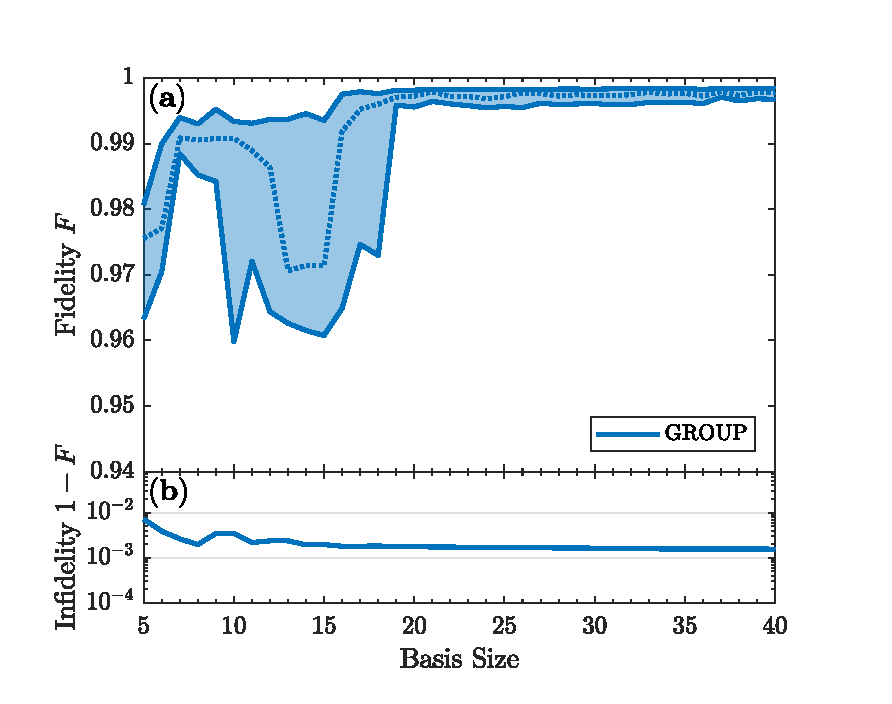
\includegraphics[width=0.45\textwidth]{Figures/FidelityBasisSize.pdf}
    \caption{\textit{Final fidelity obtained for optimal control at various optimization space dimensions for duration $T = 2.5$. \textbf{(a)} the dotted line marks the median fidelity achieved, while the shaded area displays the $25\%$- and $75\%$-quartiles of the solutions. \textbf{(b)} the lowest infidelities achieved for each basis size.}}
    \label{fig:FidelityBasisSize}
\end{figure}

\begin{figure}[h!]
    \centering
    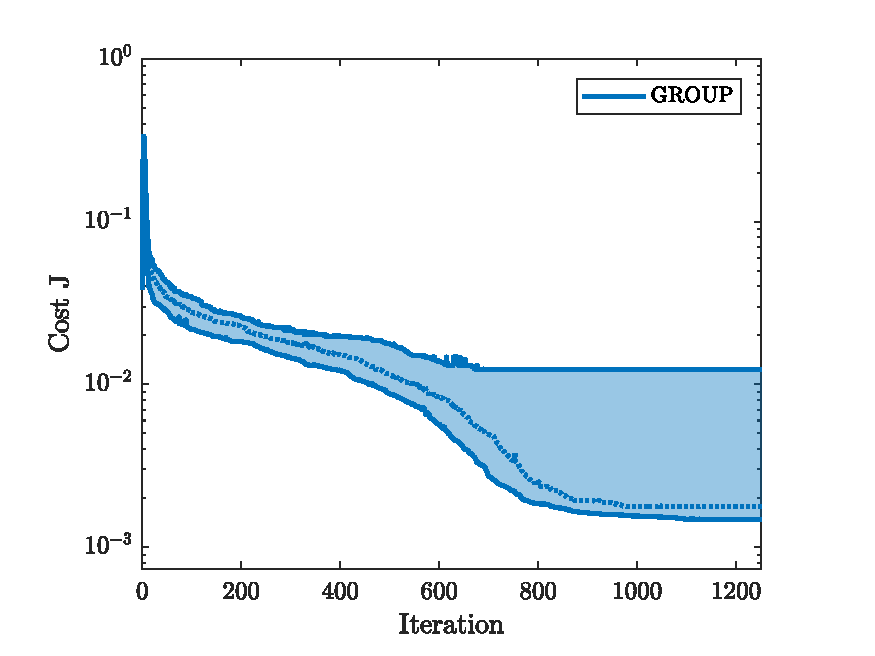
\includegraphics[width=0.45\textwidth]{Figures/CostProgress.pdf}
    \caption{\textit{The value of the cost function at a given number of time evolutions. The dotted line marks the median and the shaded area indicates the $25\%$- and $75\%$-quartiles found from X different random initial controls.}}
    \label{fig:FidelityBasisSize5}
\end{figure}


%\bibliographystyle{apsrev4-1}
\bibliography{references.bib}

\end{document}
%
% ****** End of file apssamp.tex ******
